\part{Realsense Camera}
\label{part:rscam}
%%%%%%%%%%%%%%%%%%%%%%%%%%%%%%%%%%%%%%%%%%%%%%%%%%%%%%%%%%%%%%%%%%%%%%%%%
%   Realsense Camera with Unity and Android                             %
%%%%%%%%%%%%%%%%%%%%%%%%%%%%%%%%%%%%%%%%%%%%%%%%%%%%%%%%%%%%%%%%%%%%%%%%%
\section{Motivation and background}
Surewash's current product range is successful in what it does, but they have key limitations. For the {\slshape ELITE} and {\slshape GO}, they are expensive, and for {\slshape Pocket}, its functionality is limited because it can only use a smartphone camera which has low resolution and is generally unpredictable. To expand Surewash's market reach, the strategy that has been adopted is to develop a cheaper version of the {\slshape GO}. At present, the core hardware in this device is a Microsoft Surface Pro, which is expensive. The core strategy therefore to reduce the cost of this device is to use another computer that is small, and cheap. One problem though is that cheap Windows devices are not that common, and when they are, they are not able to handle the workload required to run Surewash software. The core issue with hardware costs is that a Windows License and Intel processor together are expensive. A cheaper solution is to use an ARM-based device running a free operating system, such as Android.

{\slshape Pocket} was developed for Android, which is a free operating system, so it would make sense to develop this product using the Android platform, since it's well supported, and there is experience in-house with developing apps for it. Unity is used as a cross-platform framework to develop the iOS and Android variants of {\slshape Pocket}, so if Surewash was to develop using Android, Unity would be the preferred medium to develop the app with. The main issue with {\slshape Pocket}, mentioned earlier, is that it only uses a front facing mobile camera, which limits the scope for what can be seen from a Computer Vision perspective. {\slshape ELITE} and {\slshape GO} are different, they use a special camera, developed by Intel that not only gives an RGB camera feed, but also a depth feed, which says how far a particular pixel is from the camera. This camera thus provides more information that can be used to get a better insight into whether someone is washing their hands correctly, or not.

The crux of the problem that this project is meant to address is thus: find a way to get an Intel Realsense camera to work on Android, using Unity. At a first glance, this would not seem to be a particularly difficult challenge, but due to the niche nature of such a task, there wasn't much information readily available on the topic, and so it was quite involved in my opinion.

\section{Underlying concepts}
This project makes use of a combination of C/C++, Java, and C sharp code. There are some key concepts that distinguish these languages, which is core to understanding how the end solution works, as well as understanding the performance of the overall solution.
    \subsection{Definitions}
        \subsubsection{Compiler} A compiler is a programme that converts code written in one language, into code of another language. This frequently implies the conversion of human-readable code such as C to machine code, such as X86 machine code, but it can also be to other languages.
        \subsubsection{Virtual Machine (VM)} A VM is a programme that emulates the hardware of a computer system. In the context of this project, VM shall refer specifically to a Process Virtual Machine, which is a programme that executes programmes in a platform-independent manner.
        \subsubsection{Ahead-Of-Time Compilation (AOT)} AOT is the concept of compiling computer code from one language into native machine code before it is run. For example, if a programme is running on an X86 processor, the AOT compiler would compile the computer code into native X86 instructions and package it into some file containing the relevant binary instructions for execution at a later time.
        \subsubsection{Just-In-Time Compilation (JIT)} JIT is the concept of compiling computer code from one language into native code during the execution of a programme.
        % \paragraph{Execution Model} specifies the behavior of a programming language.
        % \paragraph{Runtime environment}
        \subsubsection{Bytecode} Bytecode is an abstract instruction set that is designed to be efficiently interpreted into native instructions. As such, it means that it can be run on any platform using a JIT or AOT compiler.
        \subsubsection{Java Virtual Machine} Java Virtual Machine is a virtual machine that executes Java bytecode using a JIT compiler.
        \subsubsection{Java Native Interface (JNI)} JNI is a specification for interfacing between native code, and Java code.
        \subsubsection{Dalvik Bytecode} Dalvik bytecode is stored in a .DEX file and is compiled from Java Bytecode. It was originally executed in a JIT called Dalvik on Android, but this is no longer the case in modern versions of Android. 
        \subsubsection{Android Runtime (ART)} is the environment in which applications are executed on Android. When installing an application on Android, ART compiles code from DEX format to native machine code. See \cite{androidart}.
        % \subsubsection{Name mangling}
        % \subsubsection{Geometric transformation} According to \cite[pg.84]{usiskin2003mathematics}, "A geometric transformation is a function whose domain and range are sets of points. Most often the domain and range of a geometric transformation are both R2 or both R3. Often geometric transformations are required to be 1-1 functions, so that they have inverses". In the context of image processing, it can be used among other things to: translate, rotate, scale, and skew an image.

    \subsection{Programming Languages}
        \subsubsection{Java}
        Java, alongside Kotlin (which isn't used in this project), is the main programming language for writing Android applications. It is general-purpose, class based, and object-oriented. It was one of the first languages to introduce the concept of "compile once, run anywhere", meaning that its compiled code can run on any platform, regardless of processor architecture, since the compiled code, bytecode, is run in an abstract virtual machine. Its syntax is largely influenced by C++, but it doesn't have access to low-level memory facilities, instead, it is garbage collected. While the Java code is compiled to Java bytecode for Android, it isn't executed in a Java virtual machine, see the section on Android Runtime.
        \subsubsection{C}
        C is a general-purpose, imperative programming language. Its instructions map very closely to typical machine instructions, which means that it can execute fast (in comparison to code like that of Python), especially when compared to Java. C is needed in this project because JNI does not support C++ name mangling.
        \subsubsection{C++}
        C++ is built on top of C, and supports most of the features of C. It extends C by adding support for object oriented programming, generics, a standard template library for common algorithms, cross-platform thread support, and optional memory management.
        \subsubsection{C sharp}
        C sharp is similar to Java in many ways. It is a part of Microsoft's Common Language Infrastructure (CLI) specification which allows different programming languages to execute on the same virtual machine, using the same underlying data-types which makes it easy to integrate libraries written in other CLI languages. In this project, it executes on Android using the Mono Project Runtime, which is an open-source implementation of CLI (\cite{monoproject}).

    \subsection{Programming Environments}
    The core environment of this project is the Android Operating System, and by extension, the Android Runtime. However, sitting on top of that is the Unity Game Engine.
        \subsubsection{Android}
        The Java programming language forms the core of Android applications. Android does not use a Java Virtual Machine, and as such, it does not implement the full standard library of Java. Android instead has two different variants of runtimes for executing Java code. Firstly, Dalvik, a virtual machine, which is now deprecated. Dalvik was designed with mobile development in mind. Originally, when Android was being developed in the mid-2000s, mobile devices were very limited in processing power and RAM. Java bytecode is translated to Dalvik bytecode, which is then run in a JIT compiler at runtime. Modern Android devices use the Android Runtime, which also takes in Dalvik Bytecode, but it then compiles this to native code when the application is being installed (i.e. it uses AOT compilation). This uses more storage space than Dalvik, but also means that it executes faster.

        In the context of this project, it is an important consideration, since the Odroid board officially supports Android KitKat, which still uses the Dalvik VM. There was an unofficial distribution of Android Nougat (which is a more recent version of Android) for the Odroid XU4 which does use ART, which I opted for instead, since the Realsense library is CPU-intensive, and the additional overhead of the Surewash software means that any potential performance gain is crucial.
    
        \subsubsection{Unity}
        Unity is primarily a game engine, designed for writing modern 3D games. While the engine itself is written in C++, the end programmer writes C sharp scripts for game logic. The execution of C sharp is similar to Java's in so far as they are both compiled to bytecode, which is then executed in a VM. Unity uses the Mono Framework to execute C sharp code.
    
    \subsection{Hardware}
        \subsubsection{Intel Realsense D435}
        This is the camera that Surewash uses to monitor the user washing their hands, pictured in Figure \ref{fig:rs_cam}. It produces two different kinds of data feeds which can be used in conjunction with each other. Firstly, it produces an up to 1920x1080 pixel RGB feed at up to 30 frames/second at a field-of-view of 69.4 degrees x 42.5 degrees x 77 degrees. It also has a feed of depth pixels at a resolution of up to 1280x720 pixels at up to 90 frames/second and a field-of-view of 87 degrees x 58 degrees x 95 degrees. It transfers both of these feeds concurrently through a USB‑C 3.1 Gen 1 connection. See (\cite{d435}) for more information.
        \begin{figure}[h]
            \centering
            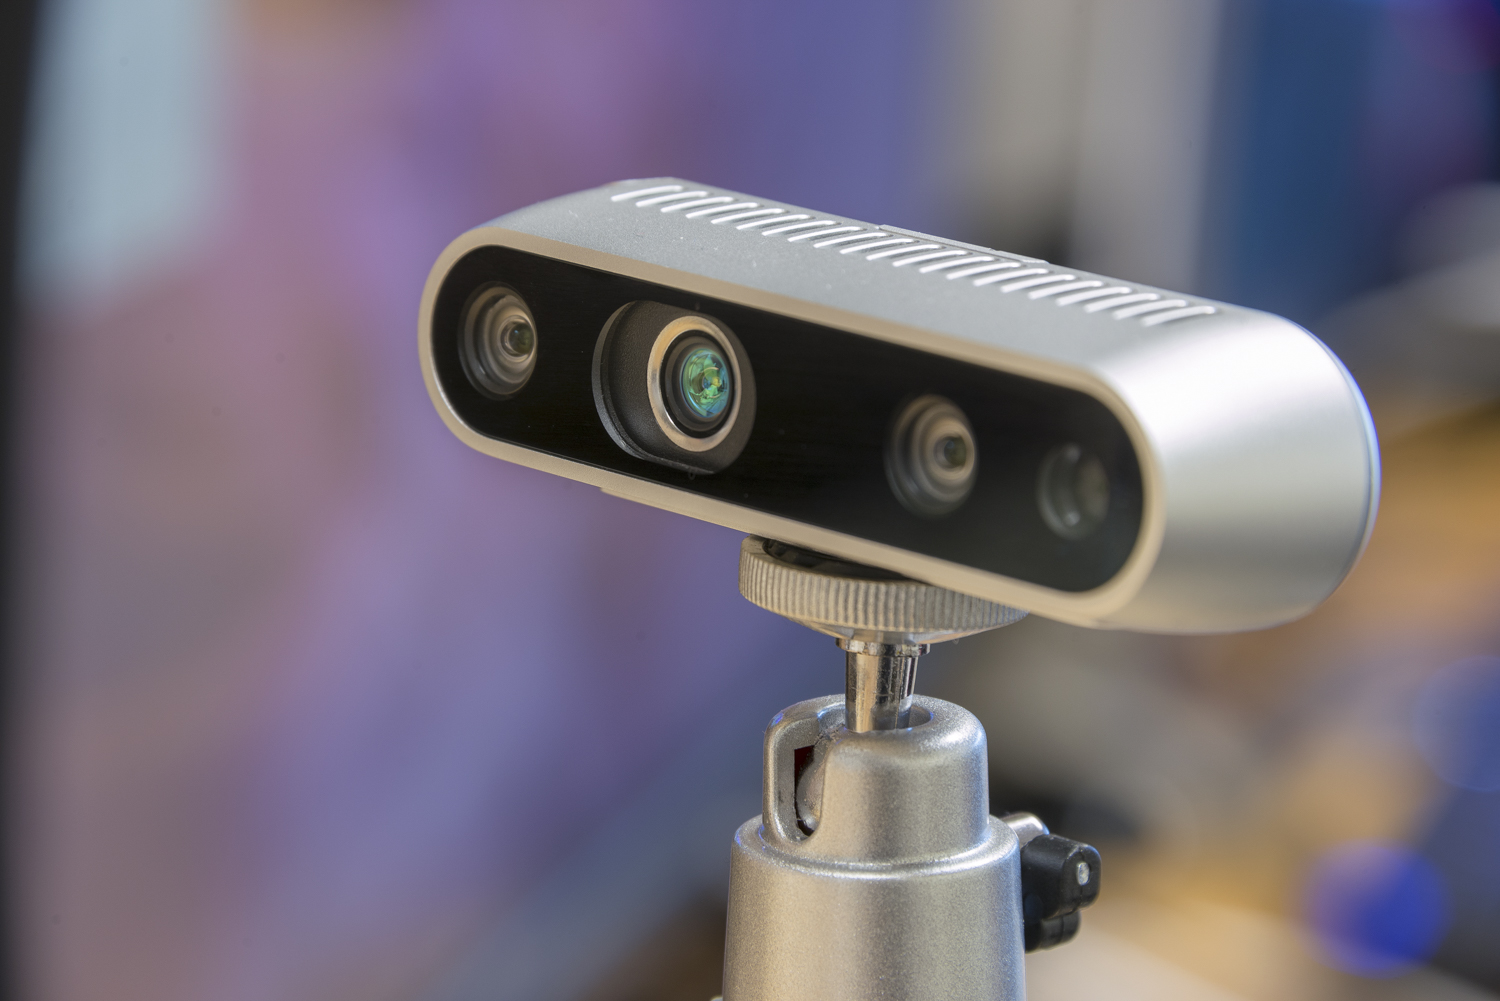
\includegraphics[height=100pt]{../img/rs_cam_2.jpg}
            \caption[]{Intel Realsense D435\footnotemark}
            \label{fig:rs_cam}
        \end{figure}
        \footnotetext{Obtained from: https://finance.yahoo.com/news/intel-realsense-depth-camera-d415-161526092.html (accessed: 30-07-2019)}

        \subsection{Hardkernel Odroid XU4}
        This is a single board computer (pictured in Figure \ref{fig:odroid}), similar in concept to a Raspberry Pi, but with a faster CPU \cite{odroid_xu4}. It contains a Samsung Exynos5 Octa SOC which contains an quad-core ARM Cortex-A15 2Ghz CPU and a quad-core ARM Cortex-A7 1.3GHz. It has 2GB of LPDDR3 RAM at 933MHz. Crucially, it contains a USB 3.0 hub which is required to interact with the Intel Realsense camera. It contains a relatively large heatsink which improves performance since it reduces the need for thermal throttling.

        \begin{figure}[h]
            \centering
            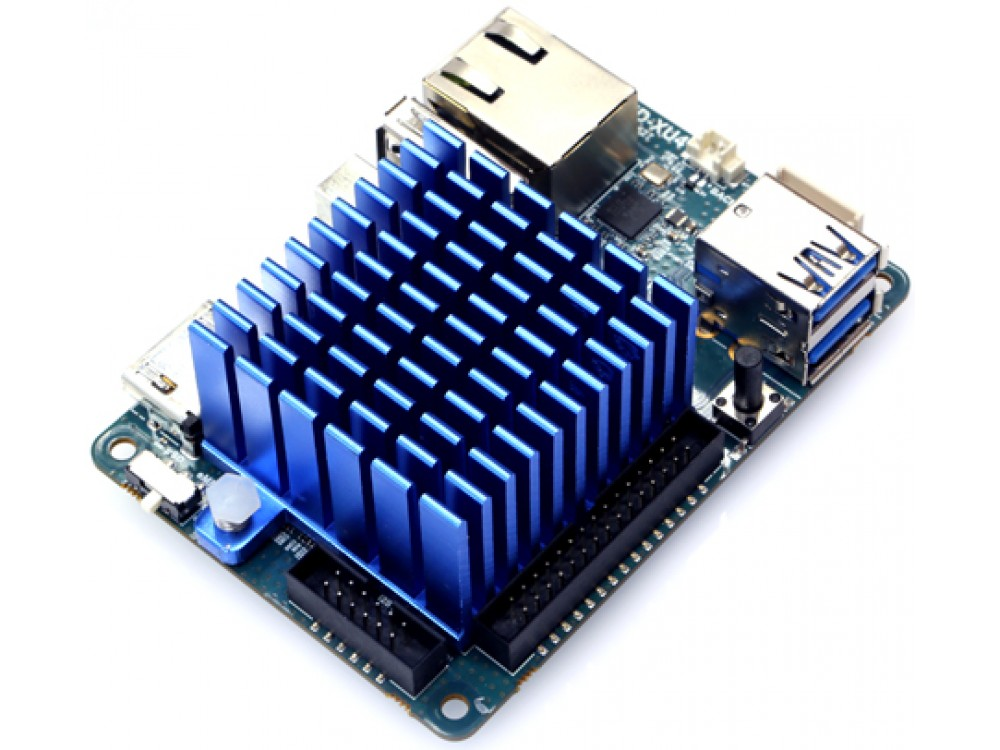
\includegraphics[height=100pt]{../img/odroid.jpg}
            \caption[]{Odroid XU4\footnotemark}
            \label{fig:odroid}
        \end{figure}
    
    \subsection{Software}
        \subsubsection{Git}
        This is a GPL-licensed programme that allows software developers to coordinate work by hosting code in a distributed version control system. It allows developers to work on source code independently and then merge the codebase. It also allows for tracking of different files.
        \subsubsection{GitHub}
        The library for the Realsense camera is hosted in source code format on a website called GitHub. The code can be accessed on the website either using a web browser and downloading the code, or by using Git to clone the repository.
        \subsubsection{Intel Realsense Library}
        Provides a list of APIs to interact with the Realsense camera in both C and C++. It also provides software wrappers containing starter code for various platforms including Android, Unity, Windows, Python et cetera. It has an Apache v2 license.
        \footnotetext{Obtained from: https://dn.odroid.com/homebackup//201506171531272562.jpg (accessed: 30-07-2019)}

\section{The solution}
    On a high level, the solution involves making an API calling sequence to the Realsense library to produce a texture, and Unity then renders this texture. There are two threads in operation, using a producer-consumer model. The camera thread is the producer thread, and it is operating within the Realsense library, polling the camera for data and filling a buffer with frames. The Unity thread acts as the consumer, taking data from the buffer and rendering it as a texture. With the current setup, the camera produces frames faster than Unity can consume them, and since the aim is to display a live video feed, the extra data produced by the camera that Unity cannot display in time needs to be discarded, or else the buffer becomes full and the whole system crashes.

    \subsection{Realsense C API sequence}
    The Unity codebase does not interact directly with the Realsense C API, instead the relevant calls are done through Java code which makes calls to the Realsense library using JNI. The Java code is packaged into an Android library, which Unity then makes relevant calls to. This is because certain OS calls are required to allow a USB device to correctly interface, it may have been possible to have a cleaner solution, but given the time constraints on the project, this proved to be a workable solution.

    For every method mentioned below, an error variable can be passed in, which if not NULL after the function call, can be passed into an error handler which returns an enumerated error type, which can be any of the following:

    \begin{lstlisting}[style=CStyle]
typedef enum rs2_exception_type
{
    RS2_EXCEPTION_TYPE_UNKNOWN,
    RS2_EXCEPTION_TYPE_CAMERA_DISCONNECTED,      /**< Device was disconnected, this can be caused by outside intervention, by internal firmware error or due to insufficient power */
    RS2_EXCEPTION_TYPE_BACKEND,                  /**< Error was returned from the underlying OS-specific layer */
    RS2_EXCEPTION_TYPE_INVALID_VALUE,            /**< Invalid value was passed to the API */
    RS2_EXCEPTION_TYPE_WRONG_API_CALL_SEQUENCE,  /**< Function precondition was violated */
    RS2_EXCEPTION_TYPE_NOT_IMPLEMENTED,          /**< The method is not implemented at this point */
    RS2_EXCEPTION_TYPE_DEVICE_IN_RECOVERY_MODE,  /**< Device is in recovery mode and might require firmware update */
    RS2_EXCEPTION_TYPE_IO,                       /**< IO Device failure */
    RS2_EXCEPTION_TYPE_COUNT                     /**< Number of enumeration values. Not a valid input: intended to be used in for-loops. */
} rs2_exception_type;\end{lstlisting}

    First, a `context' needs to be created, among other things, this ensures that the correct API version is being used for the camera being used.
    \begin{lstlisting}[style=CStyle]
rs2_context* rs2_create_context(int api_version, rs2_error** error);\end{lstlisting}

    A `pipeline' can then be created using this `context'. This creates a new thread than handles all relevant interfacing with the camera.

    \begin{lstlisting}[style=CStyle]
rs2_pipeline* rs2_create_pipeline(rs2_context* ctx, rs2_error ** error);\end{lstlisting}   

    If a pipeline is created, it does not start actual streaming from the device. This is done with one of the following methods. The first method starts streaming without any configuration, i.e. it will use all stream types and use a default resolution, and framerate. These can be configured however and optimised for the particular setup, and this is desirable in the context of this project since a low-powered device, with a low screen resolution is being used, where a high framerate is not necessary. The configuration should be deleted after starting the pipeline.

    \begin{lstlisting}[style=CStyle]
// Start a pipeline
rs2_pipeline_profile* rs2_pipeline_start(rs2_pipeline* pipe, rs2_error ** error);
rs2_pipeline_profile* rs2_pipeline_start_with_config(rs2_pipeline* pipe, rs2_config* config, rs2_error ** error);

// Creating a pipeline configuration
rs2_config* rs2_create_config(rs2_error** error);
void rs2_delete_config(rs2_config* config);
void rs2_config_enable_stream(rs2_config* config,
    rs2_stream stream,
    int index,
    int width,
    int height,
    rs2_format format,
    int framerate,
    rs2_error** error);\end{lstlisting}

    The \inlinecode{CStyle}{rs2_wait_for_frames} method can now be called. This method allocates a block of memory for a set of time-synchronised frames from the camera. What the set contains depends on the type of configuration, e.g. if only the depth and colour streams were selected, \inlinecode{CStyle}{rs2\_frame*} will point to two frames. The individual frames can then be extracted using the \inlinecode{CStyle}{rs2\_extract\_frame} method, providing an integer index. The type of frame must then be determined using the \inlinecode{CStyle}{rs2\_get\_stream\_profile\_data} method, the first parameter {\slshape mode} is found by calling \inlinecode{CStyle}{rs2\_get\_frame\_stream\_profile}, the second parameter is the \inlinecode{CStyle}{rs2\_frame*} value, the other parameters are output values for information about the frame.

    \begin{lstlisting}[style=CStyle]
// Get individual frames
rs2_frame* rs2_pipeline_wait_for_frames(rs2_pipeline* pipe, unsigned int timeout_ms, rs2_error ** error);
rs2_frame* rs2_extract_frame(rs2_frame* composite, int index, rs2_error** error);

// Discover type of frame
const rs2_stream_profile* rs2_get_frame_stream_profile(const rs2_frame* frame, rs2_error** error);

void rs2_get_stream_profile_data(const rs2_stream_profile* mode, 
    rs2_stream* stream, 
    rs2_format* format, 
    int* index, 
    int* unique_id, 
    int* framerate, 
    rs2_error** error);\end{lstlisting}

    For each frame from the set of frames, the following method is called to locate the raw data of the frame. The size of the data is determined by finding the product of \inlinecode{CStyle}{rs2\_get\_frame\_width}, \inlinecode{CStyle}{rs2\_get\_frame\_height}, and \inlinecode{CStyle}{rs2\_get\_frame\_bits\_per\_pixel}. The format of the data should be known when the \inlinecode{CStyle}{rs2\_get\_stream\_profile\_data} method was called, so, for example, if the format is RGBA8, each pixel will be four bytes wide (one byte per channel for red, blue, green, and alpha), and if the resolution is 1920x1080, the pointer returned by \inlinecode{CStyle}{rs2\_get\_frame\_data} will point to a block of memory 8,294,400 bytes large.

    \begin{lstlisting}[style=CStyle]
const void* rs2_get_frame_data(const rs2_frame* frame, rs2_error** error);
int rs2_get_frame_width(const rs2_frame* frame, rs2_error** error);
int rs2_get_frame_height(const rs2_frame* frame, rs2_error** error);
int rs2_get_frame_bits_per_pixel(const rs2_frame* frame, rs2_error** error);\end{lstlisting}

    Each frame must be released when it is no longer needed. When the camera is no longer needed for streaming, it must be explicitly stopped, and the pipeline deleted too.
    \begin{lstlisting}[style=CStyle]
void rs2_release_frame(rs2_frame* frame);
void rs2_pipeline_stop(rs2_pipeline* pipe, rs2_error ** error);
void rs2_delete_pipeline(rs2_pipeline* pipe);\end{lstlisting}

    % The algorithm that Surewash uses requires both a colour, and depth stream. It needs these streams to be the same resolution, but the Realsense camera gives these streams at different resolutions. A geometric transformation to scale one of the streams in terms of the other is therefore required to

    \subsection{Java API sequence}
    For each method described above, there is a corresponding JNI wrapper call that calls these methods. For example, the following JNI call is used to create a Pipeline instance. It is interesting to note that since Java does not support pointers in the same way as C pointers, the C pointer is stored in a Java {\slshape long} variable. This can be seen as analogous to storing a C pointer in a C {\slshape long long}, and in this case, the C compiler would throw an error, since it violates the C type system. A type system is important for disciplined and safe programming this should be avoided as \cite{pierce2002types} argues, but there is no way to avoid this within JNI.
    \begin{lstlisting}[style=CStyle]
// Copyright(c) 2015 Intel Corporation.
JNIEXPORT jlong JNICALL Java_com_intel_realsense_librealsense_Pipeline_nCreate(JNIEnv *env, jclass type, jlong context) {
    rs2_error* e = NULL;
    rs2_pipeline* rv = rs2_create_pipeline(context, &e);
    handle_error(env, e);
    return rv;
}\end{lstlisting}

    In the Java code, the JNI calls are grouped into classes based on the type data, so there is a class corresponding to a Pipeline, FrameSet, Frame etc. The following is an example of the JNI call above (note that the other methods have been removed for the sake of brevity).

    \begin{lstlisting}[style=CSharpStyle]
public class Pipeline extends LrsClass{
    public Pipeline(){
        RsContext ctx = new RsContext();
        mHandle = nCreate(ctx.getHandle());
    }
    private static native long nCreate(long context);
}\end{lstlisting}

    The {\slshape native} keyword in a function declaration says that its definition is in C code.

    The Android wrapper only contained a subset of the entire functionality of the Realsense library. One of the requirements of this project was for the ability to align a depth and colour frame. The Realsense camera does not give the depth and colour frames at the same resolution, so this functionality processes the camera feed and scales one of the feeds to the other. This functionality was not in the Android Wrapper, so this was added by putting additional JNI calls in a similar manner to Pipeline.

    \subsection{API sequence within Unity}
    Appendix \ref{appendix:rsunitysol} is the entire C sharp solution required to access the camera, {\slshape AndroidJavaObject} methods that contain `unity' denote functions that I added to the Realsense codebase to use within Unity for this project. Unity has a Java interface called {\slshape AndroidJavaObject} (\cite{unityandroidjavaobject}), this means that there is potentially an unnecessary bottleneck in that instead of calling the Realsense library directly, it is done via the Java code. This is particularly problematic given that for each colour and depth frame, they are first passed through three buffers. Firstly, a buffer within the Realsense code takes the data from the camera, this data is then copied from that buffer to a buffer within the Java code, and then the data is copied from the Java buffer into another buffer within the Unity code (see lines 56-64 below). Given that this data is uncompressed, it represents a large, potentially unnecessary overhead. In practice, this was not a problem, since a smooth frame rate was achieved, and finding a solution to that problem would have taken too much time.

    Although C sharp is a garbage-collected language, this does not extend to the {\slshape AndroidJavaObject}, so the resources have to be freed manually using the {\slshape Dispose()} method.
    

\section{Conclusion}
    \subsection{Learning Outcomes}
        \subsubsection{Programme design}
            \paragraph{Build tools}
            I learned about build tools such as Cmake, and Gradle. I learned that they are examples of programmes that can be used to automate the build process of a programme and library. I gained experience in using them, and learned about the importance of using them in large projects.
            \paragraph{Debugger}
            I learned how to use the Android debugger within Android Studio. I learned what breakpoints are, and how to use them as well logs to assist with debugging.
            \paragraph{Understanding how to read and understand other people's code}
            While I may already have a good understanding of how to programme in, say C, and C++, that doesn't necessarily mean that I have the skills to read other people's code and understand what's going on there. I learned how to trace through different function calls, and using breakpoints in a debugger to understand how a piece of code works.
    % \subsection{Reflection}
        